%%**************************************************************
%% Vorlage fuer Bachelorarbeiten (o.ä.) der DHBW
%%
%% Autor: Tobias Dreher, Yves Fischer
%% Datum: 06.07.2011
%%**************************************************************

\newcommand{\pdftitel}{Test Framework für Unity}
\newcommand{\autor}{Lennart Hensler}
\newcommand{\arbeit}{Studienarbeit}

%
% Nahezu alle Einstellungen koennen hier getaetigt werden
%

\documentclass[%
	pdftex,
	oneside,		% Einseitiger Druck.
	12pt,			% Schriftgroesse
	parskip=half,	% Halbe Zeile Abstand zwischen Absätzen.
	headsepline,	% Linie nach Kopfzeile.
	footsepline,	% Linie vor Fusszeile.
	abstracton,	    % Abstract Überschriften
	ngerman,		% Translator
]{scrreprt}

%Seitengroesse
\usepackage{fullpage}

%Zeilenumbruch und mehr
\usepackage[activate]{microtype}

% Zeichencodierung
\usepackage[utf8]{inputenc}
\usepackage[T1]{fontenc}

% Zeilenabstand
\usepackage[onehalfspacing]{setspace}

% Index-Erstellung
\usepackage{makeidx}

% Lokalisierung (neue deutsche Rechtschreibung)
\usepackage[ngerman]{babel}

% Anführungszeichen 
\usepackage[babel,german=quotes]{csquotes}
%\usepackage[style=swiss]{csquotes}


% Spezielle Tabellenform fuer Deckblatt
\usepackage{longtable}
\setlength{\tabcolsep}{10pt} %Abstand zwischen Spalten
\renewcommand{\arraystretch}{1.5} %Zeilenabstand

% Grafiken
\usepackage{graphicx}

% Mathematische Textsaetze
%\usepackage{amsmath}
%\usepackage{amssymb}

% Pakete um Textteile drehen zu können, oder eine Seite Querformat anzeigen kann.
%\usepackage{rotating}
%\usepackage{lscape}

% Farben
\usepackage{color}
\definecolor{LinkColor}{rgb}{0,0,0.2}
\definecolor{ListingBackground}{rgb}{0.92,0.92,0.92}
\definecolor{ListingKeyword}{RGB}{57, 135, 214}
\definecolor{ListingString}{RGB}{214, 136, 82}
\definecolor{ListingComment}{RGB}{84, 139, 61}
\definecolor{ScriptClass}{RGB}{192, 0, 192}
\definecolor{ScriptLogicInterface}{RGB}{0, 128, 128}
\definecolor{LogicClass}{RGB}{255, 128, 0}
\definecolor{HealthClass}{RGB}{0, 128, 0}
\definecolor{MovementClass}{RGB}{0, 0, 128}
\definecolor{AttackClass}{RGB}{192, 0, 0}

% PDF Einstellungen
%\usepackage[%
%	pdftitle={\pdftitel},
%	pdfauthor={\autor},
%	pdfsubject={\arbeit},
%	pdfcreator={pdflatex, LaTeX with KOMA-Script},
%	pdfpagemode=UseOutlines, % Beim Oeffnen Inhaltsverzeichnis anzeigen
%	pdfdisplaydoctitle=true, % Dokumenttitel statt Dateiname anzeigen.
%	pdflang=de % Sprache des Dokuments.
%]{hyperref}

% (Farb-)einstellungen für die Links im PDF
%\hypersetup{%
%	colorlinks=false, % Aktivieren von farbigen Links im Dokument
%	linkcolor=LinkColor, % Farbe festlegen
%	citecolor=LinkColor,
%	filecolor=LinkColor,
%	menucolor=LinkColor,
%	urlcolor=LinkColor,
%	bookmarksnumbered=true % Überschriftsnummerierung im PDF Inhalt anzeigen.
%}
\usepackage{hyperref}

% Verschiedene Schriftarten
%\usepackage{goudysans}
%\usepackage{lmodern}
%\usepackage{libertine}
\usepackage{palatino} 

% Hurenkinder und Schusterjungen verhindern
% http://projekte.dante.de/DanteFAQ/Silbentrennung
\clubpenalty=10000
\widowpenalty=10000
\displaywidowpenalty=10000

% Quellcode
\usepackage{listings}
\renewcommand{\lstlistingname}{Code} %Changing the label of listings
\renewcommand{\lstlistlistingname}{Codeverzeichnis} %Changing the name of the listings list
\lstloadlanguages{[Sharp]C}
\lstset{%
	language=[Sharp]C,		 % Sprache des Quellcodes
	numbers=left,            % Zelennummern links
	stepnumber=1,            % Jede Zeile nummerieren.
	numbersep=5pt,           % 5pt Abstand zum Quellcode
	numberstyle=\scriptsize, % Zeichengrösse 'tiny' für die Nummern.
	frame=lines,			 % Linie oben und unten als Rahmen
	breaklines=true,         % Zeilen umbrechen wenn notwendig.
	breakautoindent=true,    % Nach dem Zeilenumbruch Zeile einrücken.
	postbreak=\space,        % Bei Leerzeichen umbrechen.
	tabsize=2,               % Tabulatorgrösse 2
	showspaces=false,        % Leerzeichen nicht anzeigen.
	showstringspaces=false,  % Leerzeichen auch in Strings ('') nicht anzeigen.
	extendedchars=true,      % Alle Zeichen vom Latin1 Zeichensatz anzeigen.
	captionpos=b,            % sets the caption-position to bottom
	backgroundcolor=\color{ListingBackground}, % Hintergrundfarbe des Quellcodes setzen.
	basicstyle=\ttfamily\footnotesize,			  % Nichtproportionale Schrift, klein für den Quellcode
	keywordstyle=\bfseries\color{ListingKeyword}, % Keywords fett und blau
	commentstyle=\color{ListingComment},		  % Kommentare grün
	stringstyle=\color{ListingString}			  % Strings orange
}

% Glossar
\usepackage[
	nonumberlist, %keine Seitenzahlen anzeigen
	acronym,      %ein Abkürzungsverzeichnis erstellen
	%section,     %im Inhaltsverzeichnis auf section-Ebene erscheinen
	toc,          %Einträge im Inhaltsverzeichnis
]{glossaries}

% Fussnoten
\usepackage[perpage, hang, multiple, stable]{footmisc}

% Captions von Bildern
\usepackage[margin=10pt,format=hang,indention=-1.5cm,singlelinecheck=false,font=small,labelfont=bf]{caption}
\usepackage{subcaption}

% Appendix
\usepackage{appendix}

% Titel, Autor und Datum
\title{\titel}
\author{\autor}
\date{\datum}

%Weitere Kommandos
\newcommand{\TODO}[1]{\textcolor{red}{\textbf{TODO:} #1}} 

% Ab jetzt können auch Umlaute verwendet werden
\newcommand{\titel}{Test Framework für Unity}
\newcommand{\martrikelnr}{3581041}
\newcommand{\kurs}{TAI10B1}
\newcommand{\datumAbgabe}{27. Mai 2013}
\newcommand{\firma}{}
\newcommand{\firmenort}{}
\newcommand{\abgabeort}{Karlsruhe}
\newcommand{\abschluss}{Bachelor of Science}
\newcommand{\studiengang}{Studienganges Angewandte Informatik}
\newcommand{\dhbw}{Karlsruhe}
\newcommand{\betreuer}{Daniel Lindner}
\newcommand{\gutachter}{}
\newcommand{\zeitraum}{}

\makeglossaries
%
% vorher in Konsole folgendes aufrufen: 
%	makeglossaries makeglossaries dokumentation.acn && makeglossaries dokumentation.glo
%

%
% Abkürzungen --> referenz, name, beschreibung
% Aufruf mit \gls{...} oder Kurzform mit \acrshort{...}
%

\newacronym{DHBW}{DHBW}{Duale Hochschule Baden Württemberg}
\newacronym{I2CBus}{I\textsuperscript{2}C-Bus}{Inter-Integrated-Circuit-Bus}

%
% Glossareintraege --> referenz, name, beschreibung
% Aufruf mit \gls{...}
%
\newglossaryentry{Glossareintrag}{name={Glossareintrag},plural={Glossareinträge},description={Ein Glossar beschreibt verschiedenste Dinge in kurzen Worten}}


\begin{document}

	% Deckblatt
	\begin{spacing}{1}
		\begin{titlepage}
	{\begin{center}
		
\includegraphics[height=2.6cm]{images/dhbw.png}
	\end{center}}
	\enlargethispage{20mm}
	\begin{center}
		\vspace*{12mm}	{\LARGE\bf \titel }\\
		\vspace*{12mm}	{\large\bf \arbeit}\\
		\vspace*{12mm}	des \studiengang\\
		\vspace*{3mm} 	an der Dualen Hochschule Baden-Württemberg \dhbw\\
		\vspace*{12mm}	von\\
		\vspace*{3mm} 	{\large\bf \autor}\\
		\vspace*{12mm}	\datumAbgabe\\
	\end{center}
	\vfill
	\begin{spacing}{1.2}
	\begin{tabbing}
		mmmmmmmmmmmmmmmmmmmmmmmmmm     \= \kill
		\textbf{Kurs}                  \>  \kurs\\
		\textbf{Betreuer}              \>  \betreuer\\
	\end{tabbing}
	\end{spacing}
\end{titlepage}

	\end{spacing}
	\newpage

	\renewcommand{\thepage}{\Roman{page}}
	\setcounter{page}{1}

	% Erklärung
	\thispagestyle{empty}

\section*{Erklärung}
% Seite 8
% http://studium.ba-bw.de/fileadmin/media/allgemein/bestimmungen/btechnik/richtlinien/Richtlinien_Praxismodule_Studien_und_Bachelorarbeiten_2011.pdf
\vspace*{2em}

gemäß § 5 (2) der „Studien- und Prüfungsordnung DHBW Technik“ vom 18. Mai 2009.

Ich habe die vorliegende Arbeit selbstständig verfasst und keine anderen als die angegebenen
Quellen und Hilfsmittel verwendet.
\vspace{3em}

\abgabeort, \datumAbgabe
\vspace{4em}

\autor


	\newpage

	% Abstract
	\pagestyle{empty}

\renewcommand{\abstractname}{Zusammenfassung}
\begin{abstract}
Diese Studienarbeit handelt von der Entwicklung eines Frameworks automatisierter Tests für die Spiele-Engine Unity. Im Rahmen einer vorherigen Studienarbeit wurde versucht ein Spiel testgetrieben zu entwickeln. Dabei hat sich herausgestellt, dass die verhaltenssteuernden Komponenten eines Spiels nur marginal testen lassen. Aus diesem Grund möchte ich versuchen ein eigenes Framework zu entwickeln, welches einen größeren Funktionsumfang bietet. Dabei analysiere ich zunächst die schon vorhanden Frameworks, beschreibe einen möglichen Erstentwurf und anschließend die konkrete Implementierung.
\end{abstract}


\renewcommand{\abstractname}{Summary}
\begin{abstract}
Meh.
\end{abstract}

	\newpage

	\pagestyle{plain}

	% Inhaltsverzeichnis
	\begin{spacing}{1.1}
		\setcounter{tocdepth}{1}
		\tableofcontents
	\end{spacing}
	\newpage

	\renewcommand{\thepage}{\arabic{page}}
	\setcounter{page}{1}
	
	% Inhalt
	\chapter{Einleitung}
\label{sec:Einleitung}

In der Software-Entwicklung wird immer mehr Wert auf automatisierte Tests, um die Korrektheit des Programms zu gewährleisten und für die klassische Entwicklung gibt es schon mächtige Werkzeuge, die einen dabei unterstützen. Angefangen mit Test-Frameworks, welche es einem ermöglichen atomare Teile des Codes, bis zu dessen Gesamtheit automatisch zu testen, wodurch man schnelles Feedback erhält und Fehlverhalten leicht aufdecken kann. Darüber hinaus lässt sich mit Code Coverage Analysen feststellen, welche Teile des Codes durch Tests abgedeckt sind. Die Verwendung von Mocking-Frameworks ermöglicht es \textit{Mocks} (\hyperlink{DefinitionMock}{s. Unit-Tests weiter unten}) dynamisch zu erzeugen und deren Verhalten zur Laufzeit zu definieren. Dadurch lassen sich ohne viel Aufwand Teile des Codes komplett isoliert testen. Die testgetriebene Entwicklung stützt sich vollständig auf Tests, indem man zuerst den Test für die neue Funktionalität schreibt, diesen zum Durchlaufen bringen und anschließend refactored. Dadurch erhält man nahezu vollständig durch Tests abgedeckten Code, der offen für Änderungen und robust gegen Fehler ist. Mehr über TDD findet sich in \cite{FRE10}.

Für die Spiele-Entwicklung (mit Unity) gibt es noch keine oder nur sehr einfache Werkzeuge, um seinen Code effektiv zu testen. Deswegen möchte ich in dieser Studienarbeit ein eigenes Framework entwickeln, mit dem sich die verhaltenssteuernden Komponenten eines Spiels testen lassen. Dabei stütze ich mich auf die Erkenntnisse die ich mit einem Kommilitonen in einer vorherigen Studienarbeit \cite{TDGD13} gewonnen habe. Vor allem die Kapitel über die unterschiedlichen \nameref{sec:Testarten}, die Funktionsweise von \nameref{sec:Unity} und wie man aktuell \nameref{sec:Tests mit Unity} mit den vorhandenen Test-Frameworks durchführen kann, sind inhaltlich sehr ähnlich zu der vorangegangenen Arbeit. Dennoch möchte ich diese auf Grund der Nähe zum Thema dieser Arbeit nochmals aufführen.\\
Obwohl es bereits Frameworks für Unity gibt, habe ich mich dazu entschieden von Grund auf ein neues zu entwickeln welches den Titel \textit{JUUT} (\textbf{J}ust \textbf{U}nity \textbf{U}nit-\textbf{T}ests) tragen wird. Zum einen, um zu erfahren wie schwer es ist ein Test-Framework (für Unity) selbst zu schreiben und zum anderen, um dessen Struktur besser auf meine Bedürfnisse anzupassen.

Im nachfolgenden werde ich zunächst die unterschiedlichen Arten von Tests beschreiben und auf die Funktionsweise von Unity eingehen. Anschließend gebe ich einen Einblick in meine Entwicklungsumgebung.

\section{Testarten}
\label{sec:Testarten}

Tests sollen einen bestimmten Teil des Programms auf seine Korrektheit überprüfen und dabei möglichst schnell und automatisiert ablaufen. Je nachdem wie umfangreich der getestete Bereich ist und welche Kenntnisse der Test/Entwickler von der inneren Umsetzung des Programms hat, kann man diese kategorisieren.

\subsection{White- und Black-Box-Tests}

Die gröbste Einteilung ist die Unterscheidung zwischen White- und Black-Box-Tests. Dabei wird nicht der Umfang des getesteten Bereichs berücksichtigt, sondern lediglich ob der Entwickler des Tests Kenntnisse über die Implementierung der zu testenden Funktionen hat.\\
Bei White-Box-Tests ist dies der Fall. Idealerweise, sollte der Entwickler der den Produktivcode geschrieben hat auch den dazugehörigen Test implementieren. Mit dieser Art von Test werden die inneren Strukturen eines Programms überprüft. Also zum Beispiel, dass eine Methode nicht mit Parametern aufgerufen werden kann, die Fehler verursachen könnten. Hierbei wird nur getestet ob das Programm fehlerfrei abläuft und nicht ob die einzelnen Methoden das gewünschte Verhalten aufweisen.

Im Gegensatz dazu stehen die Black-Box-Tests, deren Entwickler keinerlei Kenntnisse über die Umsetzung haben sollte. Ansonsten könnten beim Schreiben der Tests Dinge implizit als erfüllt angesehen werden, die allerdings getestet werden müssen. Dadurch wäre es möglich, dass bei nachträglichen Änderungen Fehler auftreten, ohne dass ein Test fehlschlägt.\\
Black-Box-Tests sollen verifizieren, dass das Programm die Spezifikationen des Kunden erfüllt.

Diese beiden Testarten ergänzen sich gegenseitig und es sollten immer sowohl White-Box, als auch Black-Box-Tests erstellt werden, um das Produkt zu überprüfen und robust gegen Fehler bei nachträgliche Änderungen zu machen.\\
Schematische Darstellungen dieser Testarten sieht man in \autoref{fig:White_Box_Test} und \autoref{fig:Black_Box_Test} auf der nächsten Seite.

\paragraph{Grey-Box-Tests} stellen eine Mischung aus beiden Varianten dar und vereinen die Eigenschaften beider Arten. Diese erhält man zum Beispiel durch testgetriebene Entwicklung, da man den Test schreibt bevor man den Code implementiert. Dadurch kann man keinerlei Kenntnisse über dessen innere Struktur haben, sondern definiert per Test das erwartete Verhalten. Nachdem dieser erfolgreich ausgeführt wird, erweitert man ihn im Sinne von White-Box-Tests. Dadurch wird sowohl das nach außen sichtbare Verhalten, als auch die innere Struktur des Codes getestet und man benötigt nur einen Entwickler für die Tests.

\clearpage
\begin{figure}[t]
\centering
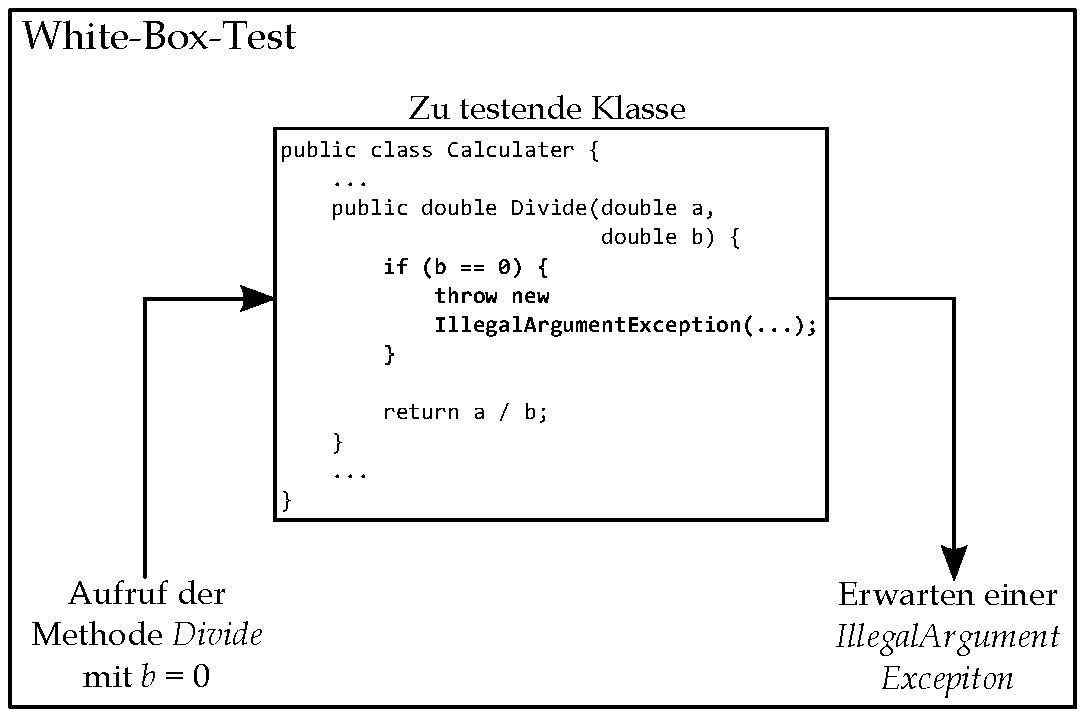
\includegraphics[width=0.8\linewidth]{./images/Kapitel_Einleitung/White_Box_Test.pdf}
\caption[Schematische Darstellung eines White-Box-Tests]{Schematische Darstellung eines White-Box-Tests\\Der Entwickler sollte sich gut mit dem zu testenden Code auskennen. Der Test verifiziert, dass die Methode korrekt ausgeführt wird.}
\label{fig:White_Box_Test}
\end{figure}

\begin{figure}[b]
\centering
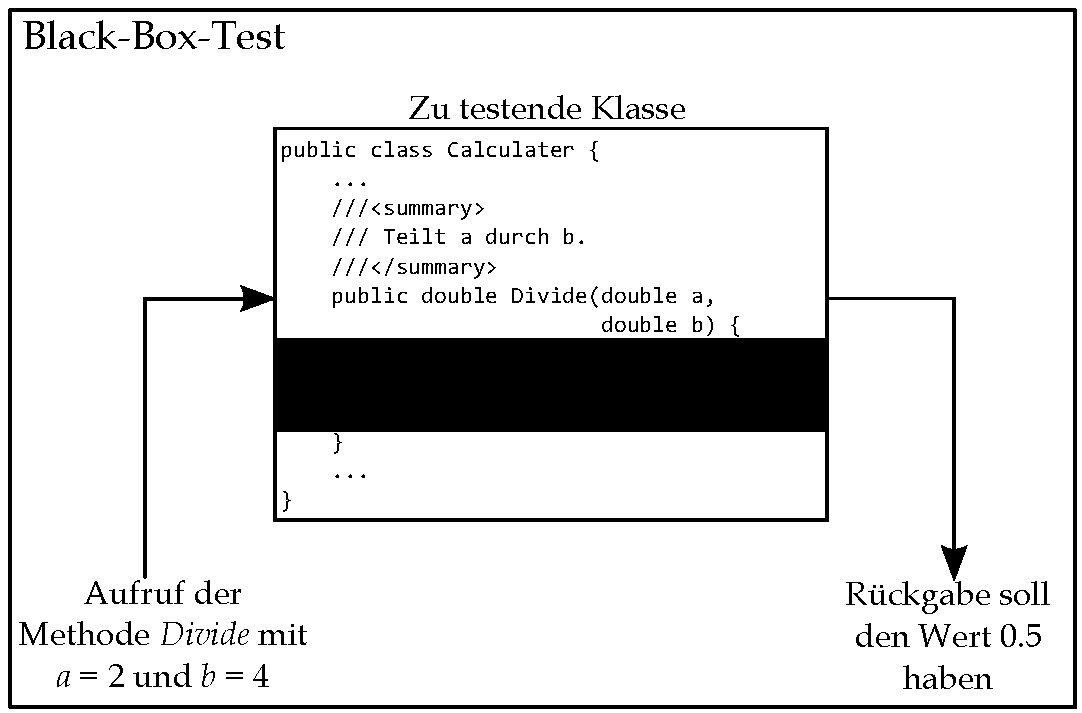
\includegraphics[width=0.8\linewidth]{./images/Kapitel_Einleitung/Black_Box_Test.pdf}
\caption[Schematische Darstellung eines Black-Box-Tests]{Schematische Darstellung eines Black-Box-Tests\\Öffentliche Klassen und Methoden, sowie deren Beschreibungen sind dem Entwickler bekannt. Die konkrete Implementierung allerdings ist nicht einsehbar. Der Test verifiziert das Verhalten der zu testenden Klasse.}
\label{fig:Black_Box_Test}
\end{figure}
\clearpage

\subsection{Unit-Tests} 

Diese sind die kleinsten Einheiten unter den Tests. Sie sollen die einzelnen Methoden einer Klasse auf einen fehlerfreien Ablauf und ein korrektes Verhalten hin testen. Dadurch kann man im Verlauf der Entwicklung Änderungen am Programm vornehmen, ohne dass die Funktionalitäten der Module unbemerkt zerstört werden, insofern die Tests eine ausreichende Abdeckung erreichen (sowohl semantisch, als auch von den Zeilen her).\\
Die einzelnen Tests sollten unabhängig voneinander und auch von den anderen Komponenten sein. Falls Verbindungen zwischen den Komponenten bestehen, sollten diese durch \hypertarget{DefinitionMock}{\textit{Mock}}-Objekte entkoppelt werden. Diese erben von der entsprechenden Klasse und überschreiben deren Methoden auf eine geeignete Art. Zum Beispiel könnten sie einfach leer gelassen werden, was man als \textit{Stub} bezeichnet. Oder sie geben einen festen Wert zurück. \textit{Mock}-Klassen können selbst erstellt werden und sind meistens innere Klassen der Testklasse, allerdings gibt es auch \textit{Mock}-Frameworks, welche generisch \textit{Mocks} für beliebige Klassen oder Interfaces erzeugen können. Das Verhalten der Methoden eines Mocks, lässt sich mit diesen zur Laufzeit festlegen. Zum Beispiel dass ein fester Wert zurückgeliefert wird, oder eine Exception geworfen werden soll.\\ Beispiele sind \textit{JMock} für Java oder \textit{Moq} für C\#.\\
Außerdem sollten Unit-Tests sehr schnell ablaufen (im Millisekunden-Bereich), um nach jeder Änderung durchgeführt werden zu können, ohne die Entwicklung aufzuhalten.

Eine schematische Darstellung von Unit-Tests sieht man in \autoref{fig:Unit_Test}.

\subsection{Integrationstests}

Die nächsthöhere Stufe von Tests sind Integrationstests. Diese testen das Zusammenspiel mehrere Komponenten, eventuell auch mit Systemressourcen, auf ihre Korrektheit. Einen Unit-Test kann man zu einem Integrationstest machen, indem man die \textit{Mock}-Objekte durch die im Produktivbetrieb verwendet Klassen ersetzt und die Bedingungen entsprechend anpasst.

Integrationstests dürfen länger dauern als Unit-Tests, sollten dennoch schnell durchgeführt werden können.

Eine schematische Darstellung von Integrationstests sieht man in \autoref{fig:Integration_Test}.

\subsection{Akzeptanztests} 

Diese sollen die Korrektheit des Verhaltens eines ganzen Systems prüfen. Dabei soll er sowohl die Benutzerschnittstelle, als auch die einzelnen Komponenten und die Systemressourcen abdecken. Allerdings testen diese nicht die innere Struktur des Systems (und sind dementsprechend Black-Box-Tests), sondern sollen gewährleisten, dass ein System sich so verhält, wie es der Kunde im Lastenheft definiert hat. Idealerweise verwendet der Test dabei nur die Schnittstellen, die ein Kunde auch verwenden würde (z.B. über Eingaben auf der GUI), um möglichst nahe an ein natürliches Verhalten zu kommen.\\
Akzeptanztests können durchaus länger dauern, da sie das gesamte Verhalten eines Systems repräsentieren, welches nur nach größeren Veränderungen getestet werden muss.

\begin{figure}[h]
\centering
	\begin{subfigure}[b]{0.29\textwidth}
	\centering
	\captionsetup{justification=centering}
	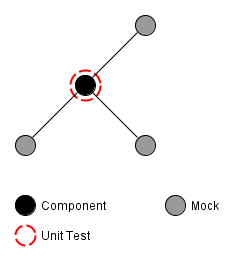
\includegraphics[width=\textwidth]{./images/Kapitel_Einleitung/Unit_Test.png}
	\caption{Unit-Test}
	\label{fig:Unit_Test}
	\end{subfigure}
	\begin{subfigure}[b]{0.29\textwidth}
	\centering
	\captionsetup{justification=centering}
	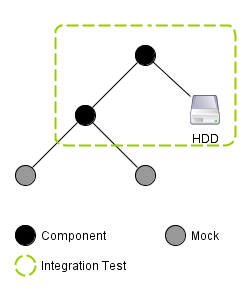
\includegraphics[width=\textwidth]{./images/Kapitel_Einleitung/Integrations_Test.png}
	\caption{Integrationstest}
	\label{fig:Integration_Test}
	\end{subfigure}
	\begin{subfigure}[b]{0.39\textwidth}
	\centering
	\captionsetup{justification=centering}
	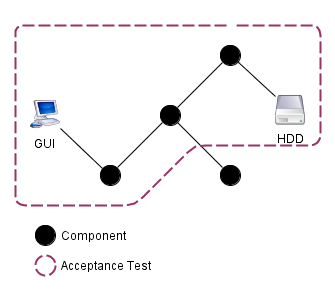
\includegraphics[width=\textwidth]{./images/Kapitel_Einleitung/Akzeptanz_Test.png}
	\caption{Akzeptanztest}
	\label{fig:Acceptance_Test}
	\end{subfigure}
\caption[Schematische Darstellung der unterschiedlichen Testarten]{Schematische Darstellung der unterschiedlichen Testarten\\(a) testet die einzelnen Methoden einer Komponente. Alle anderen benötigten Komponenten sollten als Mock-Objekte eingebunden werden.\\(b) testet das Verhalten mehrere Komponenten und eventuell im Zusammenhang mit Systemressourcen\\(c) testet einen Großteil der Komponenten eines Programms mit den Systemressourcen nach den Anforderungen des Kunden.\\
Quelle: \url{http://schneide.wordpress.com/2011/09/05/a-shot-at-definitions-beyond-unit-test/}}
\label{fig:UnitIntegrationAcceptanceTest_Comparison}
\end{figure}
\clearpage

\section{Unity}
\label{sec:Unity}

\textit{Unity} ist eine Spiele-Engine, welche für viele verschiedene Anwendungen, wie Spiele, Lernsoftware, sowie 3D-Animationsfilme verwendet wird. Der Hersteller bezeichnet die Software selber als \textit{Spieleentwicklungs-Ökosystem}\footnote{Zu lesen unter \url{http://unity3d.com/unity/}}, da sie neben der Engine selber eine komplette Entwicklungsumgebung für Spiele bietet.\\
Die Umgebung erlaubt es einem, die Spiele auch auf andere Plattformen zu portieren, wie zum Beispiel für Android auf Smartphones oder für Webanwendungen. Dies macht die Engine sehr flexibel und ist auch ein Grund für die weite Verbreitung. Der Spielecode für das Spiel lässt sich in verschiedenen Sprachen programmieren, die beim Übersetzen alle von der Unity-Umgebung in die Common Intermediate Language überführt werden, eine Assemblersprache, die erst beim Ausführen in einer Laufzeitumgebung (.NET oder Mono) in nativen Maschinencode übersetzt wird. Die verfügbaren Scriptsprachen sind JavaScript, C\# und Boo\footnote{Weitere Infos zu Boo unter \url{http://boo.codehaus.org/}}.

\subsection{Unity als Entwicklungsumgebung} 

Im Mittelpunkt steht ein Szeneneditor, der es ermöglicht die einzelnen Spielszenen zu gestalten, indem die Spielelemente in einem 3D-Editor so angeordnet werden, wie sie im späteren Spiel zu sehen sind. 
Ein Element in einer Szene wird dabei \textit{GameObject} genannt, die Elemente, die zum Einbau bereit stehen, nennt man \textit{Assets}. Ein \textit{Asset} kann dabei vieles sein: Zum Beispiel 3D-Models (\textit{Meshes}), Skripte, Texturen oder Audio-Dateien. \textit{GameObjects} lassen sich beliebig hierarchisch anordnen, um sie so zu gruppieren, oder logisch zu strukturieren. Ihnen können sogenannte \textit{Components} zugeordnet werden, welche die Eigenschaften und das Verhalten dieses Objektes beschreiben. So muss immer ein \textit{Transform}-Komponente vorhanden sein, das die Position in der Welt, sowie die Rotation und die Skalierung beschreibt. Komponenten können auch Skripte sein, die bei jedem Frame für dieses \textit{GameObject} ausgeführt werden und auf Spielereingaben oder Events reagieren. Ein Event könnte zum Beispiel eine Kollision mit einem anderen \textit{GameObject} sein, ein Mausklick und vieles andere sein. Wie dies technisch umgesetzt ist, wird später erläutert.

Mit integriert in die Unity-Umgebung ist Mono-Develop, eine alternative Entwicklungsumgebung für .NET-Sprachen, welche man direkt aus Unity aufrufen kann. Die Engine bietet die Möglichkeit, das Spiel direkt aus dem Editor übersetzen zu lassen. Dies kann mit einem richtig Build geschehen, allerdings auch für Testzwecke direkt im Editor. Dabei wird aus dem 3D-Viewport einfach die Spieleansicht. Das eignet sich gut für ein schnelles Ausprobieren der Szene, ist allerdings durch eine auf Debugging ausgelegte Kompilierung nicht so schnell, wie der endgültige Build. Am Ende sind die Skripte in einer eigenen .NET-Programmbibliothek vorkompiliert und werden so von der Engine eingebunden.

\subsection{Unity als Engine}

Unity bietet als Spiele-Engine verschiedene Mechanismen, die man bei einem Spiel benötigt. Dies ist in erster Linie eine Grafik-Engine, die die gegebenen Modelle und Texturen in ein Bild auf dem Bildschirm verwandelt. Dazu kommen Engines, die Physikberechnungen durchführen, Audio abspielen, sowie Netzwerkverbindungen für Multiplayer-Spiele bieten.\\
Diese ganzen Engines bilden den Rahmen um das entwickelte Spiel, also die eigenen Skripte, welche das Verhalten des \textit{GameObjects} bestimmen. Dafür kann man in den Skripten bestimmte Methoden implementieren, die zu unterschiedlichen Zeitpunkten von der Engine ausgeführt werden. Die genaue Reihenfolge der Abarbeitung befindet sich in einer \hyperlink{MainLoopOrder}{Liste} weiter unten. Welche Methode welchen Zweck erfüllen soll, erkennt Unity an deren Name. 

Eine Methode die nahezu als erste ausgeführt wird, ist die \textit{Start}-Methode. Diese wird genutzt um das Skript zu initialisieren und wird einmalig nach der Erzeugung des konkreten Skript-Objekts ausgeführt.

Die wichtigste Methode ist \textit{Update()}, welche von der Engine bei jedem Frame aufgerufen wird. Hier müssen alle notwendigen Berechnungen für dieses Objekt und die Änderungen der Spielwelt ausgeführt werden.
Ein sehr einfaches Beispiel für ein Objekt, das sich um die y-Achse drehen soll sieht wie folgt aus.\\

\begin{lstlisting}[caption={[Einfache Skript-Klasse mit Update-Methode]Einfache Skript-Klasse mit Update-Methode}]
public class Example : MonoBehaviour{
	public void Update(){
		transform.Rotate(0,5,0);
	}
}
\end{lstlisting}

In C\# müssen alle als Skript verwendete Klassen von \textit{MonoBehaviour} erben, um von der Engine als solche erkannt zu werden und um Zugriff auf Attribute wie \textit{transform} zu erlangen. Dieses ist eine Referenz auf die zwingend vorhandene \textit{Transform}-Komponente und lässt sich über verschiedene Methoden beeinflussen, womit man das Objekt drehen, verschieben, oder skalieren kann. Wie man in diesem Beispiel sieht, wird das Objekt bei jedem Frame um den gleichen Winkel gedreht.

Weitere Methoden behandeln die Reaktion auf Events (\textit{OnTriggerEnter/Exit/Stay}) und Kollisionen (\textit{OnCollisionEnter/Exit/Stay}) mit anderen Objekten, sowie auf bestimmte Spielereingaben (z.B. \textit{OnMouseEnter} oder \textit{OnMouseOver}). Tastatureingaben müssen in der \textit{Update}-Methode behandelt werden.\\

\begin{lstlisting}[caption={[Behandlung von Tastatureingaben]Behandlung von Tastatureingaben}]
public class Example : MonoBehaviour{
	public void Update(){
		if (Input.GetKeyDown(KeyCode.Space)) {
			//Reaction when space is pressed
		}
	}
}
\end{lstlisting}

\textit{GetKeyDown} liefert während des Bildes wahr, in dem der Spieler angefangen hat die entsprechende Taste zu drücken. Neben den Werten für normalen Tasten, gibt es auch Werte für Sondertasten wie zum Beispiel \textit{Windows}, sowie Maus- und Joystick-Tasten.

Eine weitere wichtige Methode ist \textit{OnGUI()}, in der Dinge implementiert werden, die in der zweidimensionalen Schicht über der 3D-Darstellung ablaufen sollen. Hier können zum Beispiel Menüs, Lebensanzeigen oder auch Munitions-Stände und sonstige Status-Elemente angezeigt werden. \textit{OnGUI} wird bei jedem GUI-Event aufgerufen, wenn zum Beispiel auf ein GUI-Element geklickt wird. Dies kann auch häufiger als der Aufruf von \textit{Update} stattfinden, weshalb diese Aktionen in \textit{OnGUI} verarbeitet werden müssen. Alle möglichen Methoden für Skripte findet man in der Sektion \textit{Overridable Functions} der offiziellen Unity-Referenz\footnote{\url{http://docs.unity3d.com/Documentation/ScriptReference/MonoBehaviour.html}}.
\pagebreak

\paragraph{Reihenfolge der in der Hauptschleife ausgeführten Befehle}\hypertarget{MainLoopOrder}{~}\\
{\small Quelle: \url{http://docs.unity3d.com/Documentation/Manual/ExecutionOrder.html}}
\begin{enumerate}
\item Alle \textit{Awake}-Methoden
\item Alle \textit{Start}-Methoden
\item while (Schrittweite variabel zur Renderzeit des vorangegangene Bildes)
	\begin{enumerate}[label*=\arabic*.]
	\item Alle \textit{FixedUpdate}-Methoden
	\item Physik-Simulation
	\item Ausgelöste \textit{OnTriggetEnter/Exit/Stay}-Methoden
	\item Ausgelöste \textit{OnCollisionEnter/Exit/Stay}-Methoden
	\end{enumerate}
\item Transformation und Rotation der Models
\item Ausgelöste \textit{OnMouseDown/OnMouseUp}-Methoden
\item Alle \textit{Update}-Methoden
\item Animationen werden fortgesetzt
\item Alle \textit{LateUpdate}-Methoden
\item Rendern des Bildes
\end{enumerate}
\clearpage

\section{Entwicklungsumgebung}

Das Test-Framework wird in der Sprache C\# geschrieben, wobei ich \textit{Visual Studio 2012} mit dem Plugin \textit{Resharper}\footnote{Für nähere Informationen zu Resharper siehe \url{http://www.jetbrains.com/resharper/}.} als IDE verwende. \textit{Resharper} bietet einem stark erweiterte Möglichkeiten seinen Code zu refaktorisieren, also die Struktur zu verbessern, ohne die nach außen sichtbare Funktionalität zu verändern. Außerdem ist der Test Explorer wesentlich übersichtlicher, als der von \textit{Visual Studio}. Dies ist besonders wichtig, da ich testgetrieben entwickeln werde und dadurch effizienter arbeiten kann.\\
Dazu wird die Unity SDK verwendet, mit der ich ein Beispiel-Projekt, welches mein Framework verwendet, erstelle.

Als Versionierungs-Tool wird git verwendet, wobei man bei der Versionierung von Unity-Projekten ein paar Dinge beachten muss. "Dies liegt daran, dass manche Dateien in einem Unity-Projekt nur relevant für die SDK des aktuellen Benutzers sind und die Entwicklungsumgebung des Anderen stören würden, falls sie im Repository gespeichert werden. Andererseits befinden sich unter diesen Dateien auch benötigte Information, damit das Projekt korrekt funktioniert, wie zum Beispiel welche Skripte an einem Spielobjekt angehängt sind. Deswegen gibt es die Möglichkeit (seit Version 3.5 auch für die kostenlose Variante von Unity) diese Informationen in Meta-Files abzuspeichern, die sich am selben Ort wie die eigentlichen Dateien befinden. Danach muss man noch den Ordner \textit{Library} in das Gitignore-File aufnehmen. Sollte man mehrere Unity-Projekte in einem Repository haben, empfiehlt es sich in jedem Projektordner ein separates Ignore-File anzulegen, um nicht die vollständigen Pfade zu den \textit{Library}-Ordnern angeben zu müssen. Dadurch lassen sich die Ignore-Files für die einzelnen Projekte einfach kopieren" \cite[Kapitel Entwicklungsumgebung]{TDGD13}.

Eine detaillierte Anleitung zum Verwalten eines Unity-Projekts mit externen Versionierungstools findet man unter \url{http://docs.unity3d.com/Documentation/Manual/ExternalVersionControlSystemSupport.html}.
	\chapter{Tests mit Unity}
\label{sec:Tests mit Unity}

In diesem Kapitel möchte ich untersuchen, welche Möglichkeiten es zur Zeit gibt, um seine Skripte automatisiert zu testen. Dabei zeige ich zunächst kurz, wie man sein Spiel mit dem Test-Framework der Entwicklungsumgebung testen kann. Anschließend stelle ich die Frameworks der Unity-Fangemeinde und abschließend analysiere ich die Möglichkeiten und erläutere deren Probleme.

\section{Unit Test Framework der Entwicklungsumgebung (MSTest)}

Eine Möglichkeit ist es, das Framework der Entwicklungsumgebung zu verwenden. Dies wäre in diesem Fall MSTest, welches in \textit{Visual Studio} integriert ist.\\
Hierbei ist es üblich, dass man neben dem Projekt mit dem Produktivcode ein weiteres für die Tests hat. Dadurch sind diese und das Produkt sowohl räumlich, als auch logisch voneinander getrennt.

Im Nachfolgenden wird gezeigt, wie man einen Unit-Test mit MSTest aufbaut und welche Möglichkeiten es dabei gibt.

\pagebreak
\begin{lstlisting}[caption={[Unit Test mit MSTest]Unit Test mit MSTest\\
Beispiel einer Testklasse in MSTest. Zeigt wie man ihre Testmethoden deklariert und wie sie initialisiert wird.}, label=code:UnitTestMitMSTest]
using Microsoft.VisualStudio.TestTools.UnitTesting;

namespace Test_Project {
	[TestClass]
	public class UnitTest {
		[ClassInitialize]
		public static void ClassSetUp() {
			// Code to initialize the test class
			// Is called only once BEFORE all tests
		}
		[TestInitialize]
		public void SetUp() {
			// Code to intialize the single tests
			// Is called BEFORE every test
		}
		[TestMethod]
		public void TestSomething() {
			// A test
		}			
		[TestMethod]
		public void TestSomethingOther() {
			// An other test
		}
		[TestCleanup]
		public void TearDown() {
			// Code to clean the actions of the single tests
			// Is called AFTER every test
		}
		[ClassCleanup]
		public static void ClassTearDown() {
			// Code to clean the test class
			// Is called only once AFTER all tests
		}
	}
}
\end{lstlisting}
\pagebreak

Um dem Framework zu signalisieren, dass in einer Klasse Tests vorhanden sind, braucht diese das Attribut \textit{TestClass}, welches in eckigen Klammern über dem Klassennamen angegeben wird. Die einzelnen Tests in Form von Methoden werden durch \textit{TestMethod} gekennzeichnet und dürfen nichts zurückgeben und keine Parameter erwarten. Innerhalb dieser Methoden kann man mit Hilfe der Klasse \textit{Assert} bestimmte Bedingungen festlegen, die erfüllt sein müssen. Sind sie es nicht, schlägt der Test fehl und es wird eine entsprechende Meldung angezeigt. Auch wenn eine Exception nicht gefangen wird, schlägt der Test fehl und zeigt die Nachricht der Exception an.\\
Außerdem können bestimmte Methoden vor den einzelnen Tests ausgeführt werden, um zum Beispiel benötigte Objekte zu initialisieren. Dabei unterscheidet man zwischen einem Klasseninitialisierer, der genau einmal vor dem Aufruf der ersten Testmethoden ausgeführt wird und dem Testinitialisierer, der vor jedem Aufruf einer Testmethode durchgeführt wird. Der Klasseninitialisierer muss statisch sein und wird durch das Attribut \textit{ClassInitialize} markiert. Er kann zum Beispiel genutzt werden, um eine Verbindung zu einer Datenbank aufzubauen, die von mehreren Testmethoden der Testklasse verwendet wird. Der Testinitialisierer muss mit \textit{TestInitialize} gekennzeichnet werden und könnte zum Beispiel Objekte initialisieren, die von mehreren Tests gebraucht und verändert werden. Da diese dadurch vor jedem Test neu initialisiert werden, bleiben die Tests unabhängig voneinander.\\
Entsprechend zu den Initialisierern kann man auch spezielle Methoden definieren, die nach den Tests ausgeführt werden sollen. Der Klassenbereiniger könnte die zuvor geöffnete Verbindung mit der Datenbank schließen und diese von etwaigen Testdaten befreien. Der Testbereiniger kann zum Beispiel verwendet werden, um eine Singleton-Klasse auf ihren Ursprungszustand zurückzusetzen, falls dies notwendig sein sollte.

Detailliertere Informationen über das Unit Test Framework von Microsoft erhält man auf deren MSDN-Bibliotheksseite unter \url{http://msdn.microsoft.com/de-de/library/dd264975.aspx}.

Allerdings gibt es schwerwiegende Probleme, wenn man bestimmte Unity-Klassen testen möchte. Diese werden in der Analyse weiter unter näher erläutert.

\section{UUnit}

UUnit\footnote{Weitere Informationen unter \url{http://wiki.unity3d.com/index.php?title=UUnit}} ist ein Projekt der Fangemeinde für ein rudimentäres Unit Test Framework, welches in Unity Projekten verwendet werden kann. Es wurde zunächst in \textit{Boo} geschrieben, wodurch es auch Tests in \textit{Boo} erwartet. In der neusten Version (Veröffentlicht am 21.08.2012) wurde es allerdings nach C\# portiert.
Um mit UUnit Tests ausführen zu können, muss man das Framework in sein Projekt einbinden. Da UUnit Open-Source ist kann man das gesamte Framework innerhalb des \textit{Assets}-Ordners ablegen. Alternativ könnte man das Framework auch zu einer Bibliothek kompilieren und diese als Referenz einbinden.

Testklassen von UUnit müssen von der Klasse \textit{UUnitTestCase} erben, welche die beiden virtuellen Methoden \textit{SetUp} und \textit{TearDown} zur Verfügung stellt. Diese werden vor beziehungsweise nach jeder Testmethode durchgeführt und können von den expliziten Tests überschrieben werden. Die Testmethoden werden durch das Attribut \textit{UUnitTest} gekennzeichnet und mit der Klasse \textit{UUnitAssert} können Bedingungen definiert werden, die den Test fehlschlagen lassen, sollten sie nicht erfüllt sein. Allerdings bietet diese nur sechs Arten von Bedingungen, wozu \textit{Fail}, \textit{True} und \textit{Equals} gehören. Eine \textit{NotEquals}-Bedingung gibt es zum Beispiel nicht.

Innerhalb von UUnit gibt es die Klasse \textit{UUnitTestRunner}, welche alle Tests innerhalb des Projekts ausführt und das Ergebnis ausgibt. Kopiert man die Quelldatei dieser Klasse in den Ordner \textit{Assets/Standard Assets/Editor} des Unity-Proejkt, wird sogar ein neuer Knopf in die Menüleiste der Unity SDK hinzugefügt, mit dem man alle Tests ausführen lassen kann. Möchte man die Datei nicht zu seinem Projekt hinzufügen, kann man auch folgendes Skript schreiben und einem beliebigen \textit{GameObject} anfügen.

\begin{lstlisting}[caption={[Beispiel um alle UUnit-Tests auszuführen]Beispiel um alle UUnit-Tests auszuführen\\
Muss an ein \textit{GameObject} angehängt werden, wodurch beim Start des Spiels alle Tests ausgeführt werden.}, label=code:UUnitTestRunner]
public class TestRunner : MonoBehaviour {
	public void Start() {
		UUnitTestRunner runner = new UUnitTestRunner();
		runner.RunAllTests();
	}
}
\end{lstlisting}

Die Ergebnisse des Testdurchlaufs werden auf der Konsole von Unity ausgegeben, was man in der Abbildung unten sehen kann. Dabei werden die Fehlermeldungen der fehlgeschlagenen Tests, sowie die Anzahl der durchgeführten und fehlerhaften Tests ausgegeben.

\begin{figure}[h]
\centering
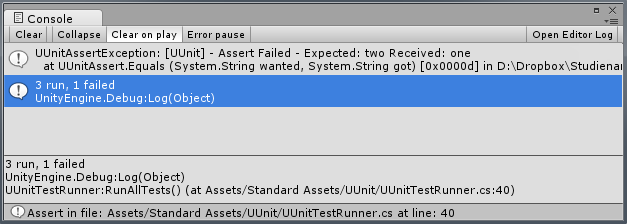
\includegraphics[width=1\linewidth]{./images/Kapitel_UnitTestsMitUnity/UUnit_Konsolenausgabe}
\caption[Ausgabe von UUnit]{Ausgabe von UUnit}
\label{fig:UUnit_Konsolenausgabe}
\end{figure}
\clearpage

\section{SharpUnit}\label{sec:SharpUnit}

SharpUnit\footnote{Weitere Informationen unter \url{http://wiki.unity3d.com/index.php?title=SharpUnit}} ist auch ein Projekt der Fangemeinde und ist in C\# implementiert. Es wurde entwickelt, da UUnit zunächst nur in \textit{Boo} zur Verfügung stand. Es orientiert sich an UUnit und hat einige Gemeinsamkeiten damit.\\
Um Tests ausführen zu können, muss man SharpUnit in sein Unity-Projekt einbinden, was wie bei UUnit funktioniert.

Testklassen müssen bei SharpUnit von der Klasse \textit{TestCase} erben, welche es ermöglicht die Methoden \textit{SetUp} und \textit{TearDown} zu überschreiben. Testmethoden werden durch das Attribut \textit{UnitTest} gekennzeichnet. Auch SharpUnit stellt einem eine Klasse zur Definition von Bedingungen zur Verfügung, wobei diese in etwa denen von UUnit entsprechen. Allerdings fehlt \textit{Fail} mit dem man einen Test geziehlt fehlschlagen lassen kann. Dafür gibt es die Möglichkeit, eine erwartete Exception zu definieren. Dies beschränkt sich allerdings auf eine pro Test, das heißt man kann keine zwei Exceptions innerhalb einer Testmethode erwarten.
 
Im Gegensatz zu UUnit können die Tests von SharpUnit nur zu Beginn des Spiels ausgeführt werden. Dafür benötigt man ein Skript, welches in der \textit{Start}-Methode bestimmte Aktionen ausführt und an ein \textit{GameObject} angehängt wird. Der nachfolgende Code ist das Beispiel von SharpUnit für so ein Skript.
\pagebreak

\begin{lstlisting}[caption={[Einbindung der Tests mit SharpUnit]Einbindung der Tests mit SharpUnit\\
Quelle: Demo von SharpUnit, erhältlich unter \url{https://github.com/mgants4/SharpUnit}.}, label=code:SharpUnitTestRunner]
public class Unity3D_TestRunner : MonoBehaviour {
	void Start() {
        // Create test suite
        TestSuite suite = new TestSuite();

        // Example: Add tests to suite
        suite.AddAll(new Dummy_Test());

        // Run the tests
        TestResult res = suite.Run(null);

        // Report results
        Unity3D_TestReporter reporter = new Unity3D_TestReporter();
        reporter.LogResults(res);
	}
}
\end{lstlisting}

Zunächst wird eine SharpUnit \textit{TestSuite} erzeugt, zu der die zu testenden Tests hinzugefügt werden. Dafür ruft man \textit{AddAll} der Suite auf und übergibt ihr eine Instanz einer Testklasse, wodurch deren Testmethoden registriert werden. Hat man die gewünschten Tests hinzugefügt, ruft man \textit{Run} der Suite auf. Diese führt die registrierten Tests aus und gibt einem Informationen über den Verlauf, in Form einer Instanz von \textit{TestResult}, zurück. Im letzten Schritt muss man einen Test-Reporter erzeugen, um damit das Ergebnis auf der Konsole der Unity SDK auszugeben. Die Ausgabe ist sehr ähnlich mit der von UUnit, zu sehen in \autoref{fig:UUnit_Konsolenausgabe}.
\pagebreak

\section{Analyse}\label{sec:Analyse}

In diesem Abschnitt werden die oben vorgestellten Frameworks bezüglich ihres Funktionsumfangs und ihrer Probleme mit Unity analysiert und verglichen. Abschließend möchte ich die meiner Meinung nach wichtigsten Kritikpunkte erläutern.

\subsection{MSTest}

Die Vorteile des von Microsoft mitgelieferten Test-Frameworks sind zahlreich. Es hat die beste \textit{Assert}-Klasse um die Bedingungen der Tests zu formulieren, da sie viele Methoden bietet. Außerdem stellt es einem als einziges die Möglichkeit zur Verfügung, einen Klasseninitialisierer/reiniger zu definieren.\\
Die Tests müssen von keiner anderen Klasse erben, sondern werden lediglich durch ein Attribut markiert. Außerdem hat man nur wenig Aufwand, um die Tests auszuführen. Das Ergebnis des Durchgangs wird nicht in der Konsole ausgegeben, sondern als Liste der einzelnen Testmethoden. Diese Liste wird in erfolgreiche, fehlgeschlagene und nicht ausgeführte Tests unterteilt. Verwendet man das Plugin \textit{Resharper} werden die Ergebnisse mit einem Baum angezeigt, was noch übersichtlicher ist.\\
Dadurch, dass MSTest unabhängig von Unity ist, sind auch die Tests unabhängig von dem Projekt. Im Gegensatz zu den anderen Frameworks, müssen sich die Tests nicht innerhalb des Unity-Projekts befinden, sondern liegen in einem separaten Projekt. Außerdem ermöglicht dies einem die Verwendung etablierter Techniken im Bereich des Testens, welche schon zu Beginn von \textit{\ref{sec:Einleitung}. \nameref{sec:Einleitung}} vorgestellt wurden.

Allerdings hat die Verwendung von MSTest auch Nachteile. Der größte ist, dass man keine Skripte - genauer gesagt keine Klassen die von \textit{MonoBehaviour} erben - testen kann, da bei deren Erzeugung eine \textit{SecurityException} auftritt, die den Test fehlschlagen lässt. Dies liegt daran, dass die \textit{MonoBehaviour} nur in einer laufenden Unity-Umgebung intialisiert werden kann. Diese lässt sich in einem Test nicht simulieren oder mocken. Um dennoch eine großflächige Abdeckung durch Tests zu erreichen, muss man die Struktur seines Projekts stark anpassen, sodass die Skripte möglichst wenig Logik enthalten. Sie müsste in eigene Klassen ausgelagert werden, wodurch sie unabhängig von Unity testbar sind. Diese Anpassung lohnt sich nur bei neuen Projekten und auch nur wenn sich das Verhalten der Objekte sinnvoll auslagern lässt. Bei einem Shooter, dessen Spielgefühl stark von einer guten Reaktion auf Benutzereingaben abhängt, ist das zum Beispiel nur schlecht möglich, da sich diese Reaktionen nicht wirklich durch einen fest definierten Test bestimmen lassen. Und auch einem speziell für diesen Fall entwickelten Projekt (dessen Prototyp im Rahmen von \cite{TDGD13} entwickelt wurde) beträgt die Abdeckung durch die Tests lediglich 45\%. Die ausgelagerte Logik hingegen erreicht eine Abdeckung von 85\%, was zeigt, dass auch bei einem Projekt bei dem sich die Logik gut auslagern lässt viel Arbeit durch die Skripte geleistet werden muss.

Was man beim Testen eines Unity-Projekts mit MSTest beachten sollte und welche Erkenntnisse dabei gewonnen wurden lässt sich in \cite{TDGD13} nachlesen.

\subsection{UUnit und SharpUnit}

Da sich diese beiden Frameworks sehr ähnlich sind, möchte ich diese gemeinsam betrachten. Der Vorteil gegenüber MSTest besteht darin, dass man auch Skripte automatisiert testen kann, da sie direkt in das Spiel eingebunden werden und somit innerhalb der Unity-Umgebung ablaufen. Allerdings benötigt man dafür ein Skript, welches für die Ausführung der Tests zuständig ist und für das ein geringer Arbeitsaufwand anfällt (s. \autoref{code:SharpUnitTestRunner} \nameref{code:SharpUnitTestRunner}). UUnit erleichtert einem das, da man über einen Menü-Punkt der Unity-SDK alle Tests ausführen lassen kann.

Dennoch kommen beide Frameworks vom Funktionsumfang nicht an MSTest heran. Hinsichtlich der Präsentation der Ergebnisse, werden diese lediglich auf der Unity Debug-Konsole ausgegeben, was bei vielen Tests schnell unübersichtlich werden kann. Außerdem gibt es keine Möglichkeit von den Testergebnissen zu der Quelldatei des Tests springen. Ein weiterer Nachteil ist, dass die Tests nun ein Teil des Unity-Projekts sind, was man bei der finalen Versionen beachten sollte, damit die Testklassen und Testszenen nicht mit ausgeliefert werden.

Eine große Einschränkung der beiden Frameworks ist, dass man nur zum Start des Spiels testen kann, da die Definition, welche Tests durchgeführt werden soll und deren Ausführung in der \textit{Start}-Methode des Skripts erfolgt. Diesen Code in die \textit{Update}-Methode auszulagern ergibt keinen Sinn, da es keine Möglichkeit gibt den Tests einen anderen Kontext zuzuordnen. Stattdessen würde die Verlagern zur Folge haben, dass die Tests bei jeder Berechnung eines Frames durchgeführt werden.

Von daher lässt sich mit den Frameworks zwar testen, dass die Skripte korrekt erstellt werden, ihre Methoden funktionieren und man ihre Attribute nicht mit unerlaubten Werten füllt. Allerdings sind Integrations- und Akzeptanztests in einem laufenden Spiel nicht möglich.

\subsection{Zusammenfassung und Kritikpunkte}

MSTest bietet von allen Frameworks die meisten Funktionalitäten und hat selbstverständlich die beste Architektur. Allerdings lassen sich damit keine Skripte oder andere Komponenten, die eine laufende Unity-Umgebung benötigen, testen. Für alles andere ist es sehr empfehlenswert.

UUnit und SharpUnit stellen einen Ansatz dar, um Skripte zu testen, aber auch nicht mehr. Die Hauptkritikpunkte sind meiner Meinung nach:
\begin{itemize}
\item \textbf{Der Aufwand zum Ausführen der Tests}\\
Dass man die auszuführenden Tests definieren muss ist kein Problem. Allerdings finde ich es unnötig, dass der Anwender die Testergebnisse selbst ausgeben muss. Ideal wäre es, wenn man nicht einmal mehr ein Skript und \textit{GameObject} zum testen benötigen würde.
\item \textbf{Fehlender Komfort der Darstellung der Ergebnisse}\\
Eine Ausgabe auf der Konsole ist nicht sehr übersichtlich und es gibt keine Möglichkeit direkt zum Fehler zu springen. Wünschenswert wäre eine Strukturierung nach Namensraum und Klasse.
\item \textbf{Geringe Auswahl an Bedingungen (\textit{Assertions})}\\
Die \textit{Assert}-Klasse bietet nur sehr wenige Methoden, um Bedingungen zu definieren. Dieses Problem lässt sich jedoch relativ leicht durch die Verwendung von \textit{NHamcrest}\footnote{\textit{NHamcrest} ist eine Bibliothek, welche einem sehr viele Assertions bietet. Es ist eine .NET-Umsetzung des in Java geschriebenen Projekts \textit{Hamcrest}. Weitere Informationen unter \url{https://github.com/grahamrhay/NHamcrest/wiki}} beheben. Allerdings werden dadurch alle fehlschlagenden Tests als Error und nicht als Fehler eingestuft, da die geworfene Exception nicht der \textit{AssertException} der Frameworks entspricht.
\item \textbf{Es sind nur simple Tests möglich}\\
Während die anderen Punkte eher kosmetischer Natur sind, stellt dieser ein echtes Problem dar, da dadurch die möglichen Tests stark eingeschränkt werden. Eine Beseitigung dieses Problems für die gegebenen Frameworks ist nicht trivial.
\end{itemize}

Im nachfolgenden gilt es nun, möglichst viele dieser Kritikpunkte zu beseitigen.
	\chapter{Konzept des Frameworks}

In diesem Kapitel wird ein möglicher Erstentwurf für das Test-Framework vorgestellt, der als Grundlage für die konkrete Implementierung dienen soll.

Zunächst betrachte ich aber die Struktur des schon existierenden Frameworks UUnit und möchte dessen Implementierung analysieren.

\section{Struktur von UUnit}

In diesem Abschnitt werde ich die Struktur von UUnit - stellvertretend für die existierenden Test-Frameworks für Unity - vorstellend und die Implementierung grob analysieren. Die daraus gewonnenen Erkenntnisse möchte ich für meinen Erstentwurf nutzen.

Auf der nächsten Seite befindet sich ein Klassendiagramm aller Klassen von UUnit und dessen relevanten Methoden. Wie man sieht besteht das Framework aus nur wenigen Klassen, wobei der Großteil der Arbeit von \textit{UUnitTestSuite} und \textit{UUnitTestCase} verrichtet wird.

\textit{UUnitTestCase} ist die Basisklasse aller Testklassen und stellt die Methoden \textit{SetUp} und \textit{TearDown} zur Verfügung, welche vor/nach jedem Aufruf eines Tests ausgeführt werden. \textit{testMethodName} repräsentiert den Namen der Testmethode, welche durch die Methode \textit{Run} gestartet werden soll. Bei der Ausführung eines Tests (s. \autoref{code:UUnitTestCase_Run} \nameref{code:UUnitTestCase_Run}) wird zunächst die \textit{SetUp}-Methode ausgeführt. Anschließend wird die auszuführende Testmethode per Reflection aufgerufen. Falls währenddessen eine Exception auftritt wird diese aufgefangen und deren Nachricht direkt über die Debug-Konsole von Unity ausgegeben. Abschließend wird \textit{TearDown} ausgeführt. Im Zuge dessen wird auch das übergebene \textit{UUnitTestResult}-Objekt aktualisiert, wobei die Anzahl der ausgeführten und fehlgeschlagenen Tests angepasst wird.

\clearpage
\begin{figure}
\centering
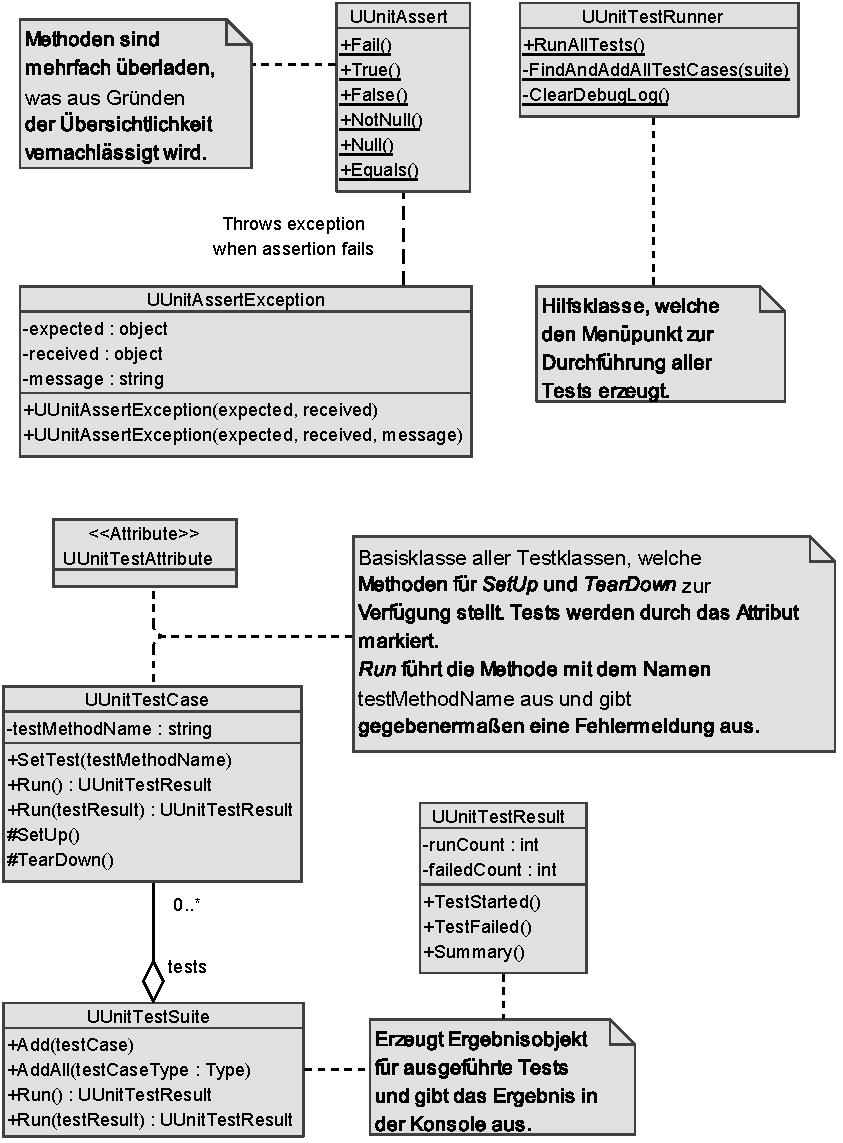
\includegraphics[width=0.9\linewidth]{images/Kapitel_ErstentwurfDesFrameworks/UUnitStruktur}
\caption[Struktur des Test-Frameworks UUnit]{Struktur des Test-Frameworks UUnit}
\label{fig:UUnitStruktur}
\end{figure}
\clearpage

\textit{UUnitTestSuite} verwaltet eine Menge von Testklassen, die per \textit{Add} und \textit{AddAll} hinzugefügt werden können. Aus dem Quellcode (s. \autoref{code:UUnitTestSuite_AddAll} \nameref{code:UUnitTestSuite_AddAll}) der \textit{AddAll}-Methode geht hervor, dass für jede einzelne Testmethode eine Instanz von \textit{UUnitTestCase} benötigt wird. Wird nun die \textit{Run}-Methode aufgerufen, wird zunächst eine \textit{UUnitTestResult}-Instanz erzeugt. Anschließend wird von jedem enthaltenen \textit{UUnitTestCase} die \textit{Run}-Methode aufgerufen, wobei das Ergebnis-Objekt übergeben. Dieses wird abschließend an den Aufrufer zurückgegeben.

Ich halte es für unnötig, dass für jede einzelne Testmethode eine Instanz der Testklasse benötigt wird, sondern denke dass eine Instanz pro Testklasse logischer wäre. Außerdem ist ein leichtes Hinzufügen weiterer Tests nur über die \textit{AddAll}-Methode möglich, da die Methode zum Hinzufügen einer einzelnen Testmethode einen Parameter vom Typ \textit{UUnitTestCase} erwartet. Dadurch muss der Anwender eine Instanz seiner konkreten Testklasse erzeugen und das Attribut \textit{testMethodName} korrekt füllen, um einen einzelnen Test hinzuzufügen. Diesen Umstand halte ich für nicht intuitiv. Des Weiteren denke ich, dass die Ausführung aller für Tests relevanten Methoden in einer separaten Klasse besser aufgehoben wäre und nicht in \textit{UUnitTestCase} gehört, da diese bereits zur Definition von Testklassen genutzt wird. Auch die direkte Ausgabe auf die Konsole, nachdem ein Test fehlgeschlagen ist sollte ausgelagert werden, um die Verantwortlichkeiten von \textit{UUnitTestCase} möglichst gering zu halten.

Diese Kritikpunkte und die geringe Größe von UUnit stützen meine Entscheidung bei der Entwicklung eines eigenen Frameworks von vorne zu beginnen.

\section{Erstentwurf für JUUT}

In der testgetriebenen Entwicklung ist es üblich vor der Implementierung ein kleines Klassendiagramm zu erstellen, in dem der Kernfunktionalität des Projekts deutlich wird \cite[Seite 32-37]{FRE10}. Mit diesem \textit{\glqq Skelette"} als Basis kann das Programm Stück für Stück erweitert werden. Das entsprechende Diagramm für mein Framework befindet sich auf der nächsten Seite und wird im folgenden erläutert.
\pagebreak

\begin{figure}
\centering
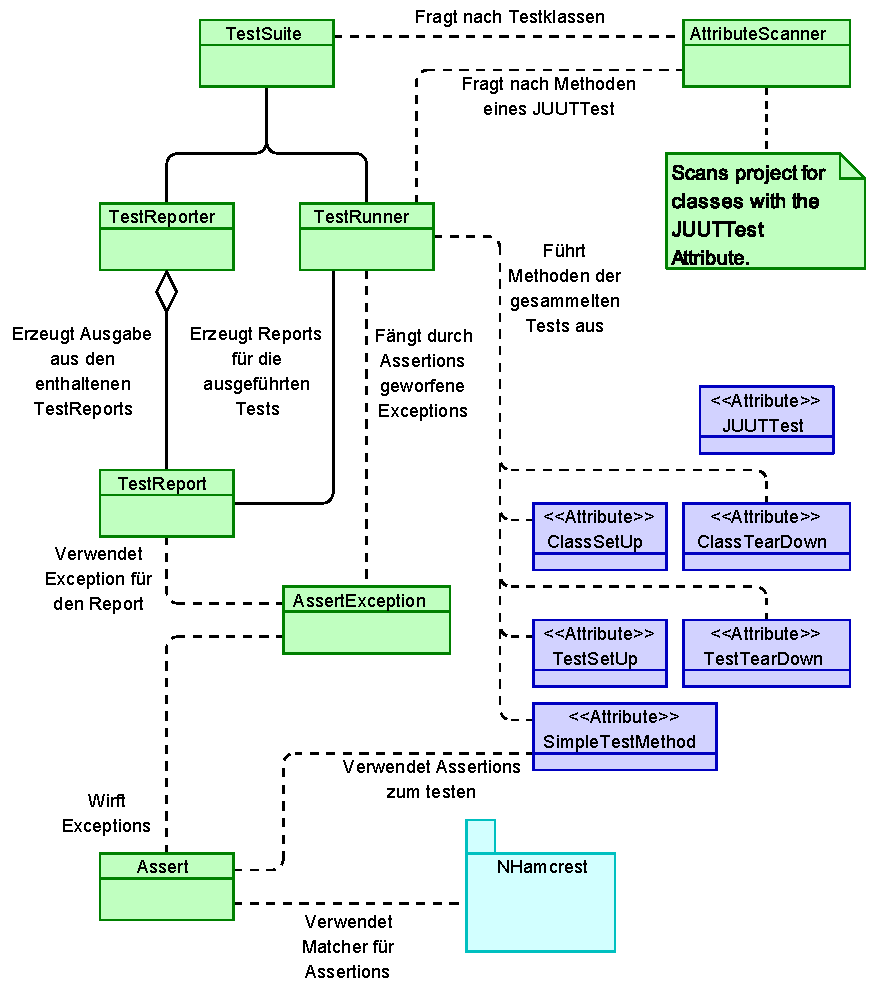
\includegraphics[width=0.9\linewidth]{images/Kapitel_ErstentwurfDesFrameworks/WalkingSkeleton}
\caption[Erstentwurf von JUUT]{Erstentwurf von JUUT}
\label{fig:WalkingSkeleton}
\end{figure}
\clearpage

Um den Aufwand für eine eigene \textit{Assert}-Klasse möglichst gering zu halten, werde ich die oben erwähnte Bibliothek NHamcrest in mein Projekt einbinden. Dabei bin ich hauptsächlich an den \textit{Matchern} interessiert, mit denen man Bedingungen, wie zum Beispiel (Un)Gleichheit zweier Objekte oder eine erwartete Exception, für die Tests definieren kann. Im Zusammenhang damit steht die \textit{AssertException}, die von \textit{Assert} geworfen werden soll, wenn eine solche Bedingung nicht erfüllt ist. Diese spezielle Exception soll einen fehlgeschlagenen Test markieren. Wird während des Tests eine andere Exception geworfen soll das als schwerer Fehler interpretiert werden.

Die Attribute dienen dazu für das Framework relevante Klassen und Methoden zu markieren, wobei ich mich an MSTest orientiert habe. Auch bei JUUT sind Attribute für \textit{Class/TestSetUp}, {Class/TestTearDown}, Testmethoden und Testklassen vorgesehen. Das Attribut zur Markierung von Tests heißt hier \textit{SimpleTestMethod}, da für die konkreten Implementierung weitere Test-Attribute geplant sind, die komplexere Tests markieren sollen. Das simple Attribut ist vergleichbar mit den Tests die in UUnit oder SharpUnit möglich sind.
Neben \textit{Assert} als statische Hilfsklasse gibt es noch den \textit{AttributeScanner}. Dieser soll zum einen dazu dienen bestimmte Methoden einer Testklasse zu finden und zurückzugeben und zum anderen wäre es vorstellbar, dass er die aktuelle Umgebung nach Testklassen durchsucht. Damit ließen sich recht einfach alle Tests des aktuellen Projekts ausführen.

Der funktionale Teil besteht aus den Klassen \textit{TestSuite}, \textit{TestRunner}, \textit{TestReporter} und \textit{TestReport}. Der \textit{TestRunner} soll eine bestimmte Testklasse verwalten und ausführen, an deren Methoden er mit Hilfe des \textit{AttributeScanners} gelangt. Wird während der Ausführung eine Exception geworfen, soll diese gefangen werden und ein entsprechender \textit{TestReport} wird erzeugt. Die \textit{TestSuite} ist die Schnittstelle für den Anwender, denn hier sollen die auszuführenden Tests hinzugefügt werden. Daraufhin werden die einzelnen \textit{TestRunner} ausgeführt und deren Reports an den \textit{TestReporter} übergeben. Abschließend wird von diesem aus den gesammelten Reports eine entsprechende Ausgabe erzeugt und angezeigt.

Dieses Konzept beseitigt die oben genannten Probleme der Implementierung von UUnit, denn die Verantwortlichkeiten sind sauber verteilt und die Komplexität wird mit Hilfe der Klasse \textit{TestSuite} vor dem Anwender verborgen.
	\chapter{Umsetzung}
	\chapter{Ergebnis}

In diesem Kapitel wird die konkrete Implementierung meines Test-Frameworks JUUT vorgestellt. Wie man in dem Übersichtsdiagramm auf der nächsten Seite sehen kann, besteht es aus einem Kernel (\textit{Core}) und einem Unity spezifischen Teil auf die ich in den nächsten zwei Sektionen eingehen werde. Zuletzt fasse ich das Erreichte kurz zusammen und vergleiche es mit den existierenden Frameworks.

Im Großen und Ganzen ist die fertige Struktur ähnlich zum \hyperref[fig:WalkingSkeleton]{Erstentwurf} abgesehen davon, dass es einen extra Bereich für die Unity spezifischen Komponenten gibt. Wodurch der Kernel auch für Test-Frameworks andere Spiele-Engines genutzt werden könnte. Das was im Erstentwurf Klassen waren, sind in der fertigen Implementierung meistens eigene Pakete, die die vorgesehene Funktionalität kapseln. Dadurch ist das Projekt offen für Erweiterungen.

\clearpage
\begin{figure}
\centering
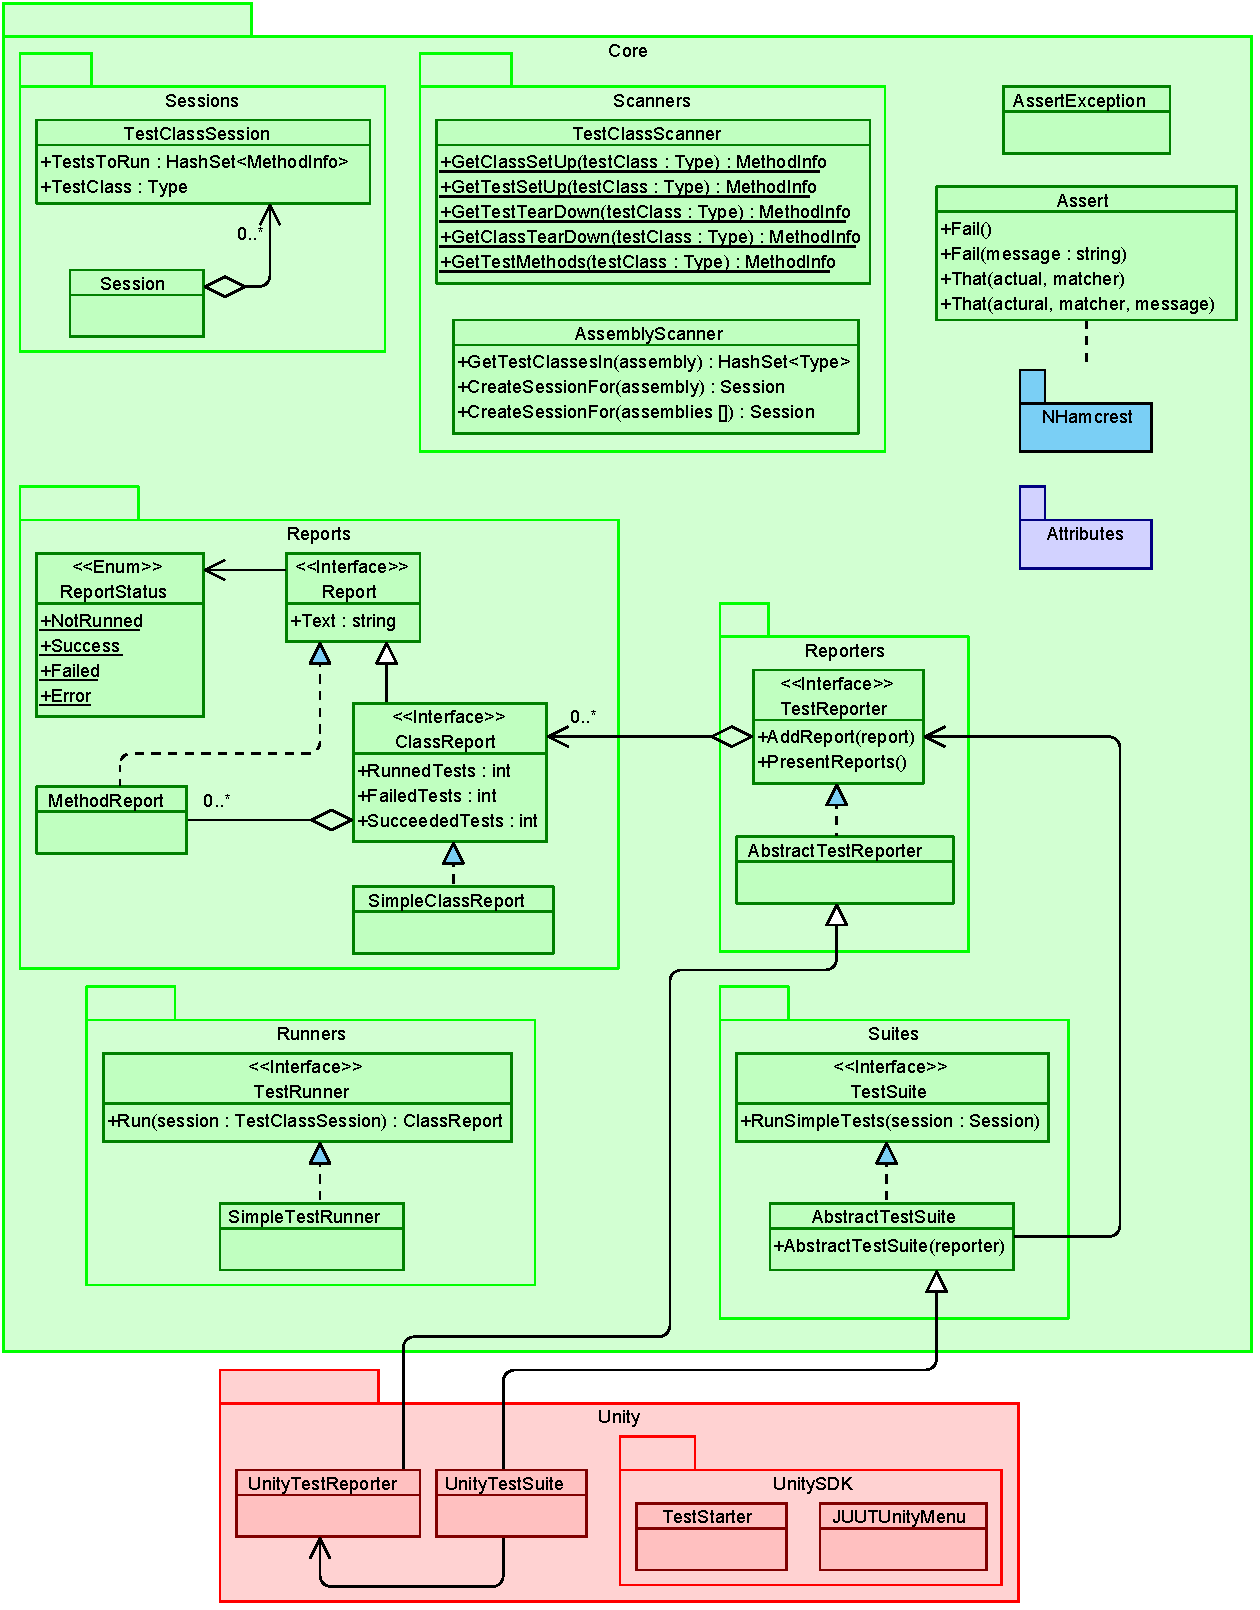
\includegraphics[width=0.9\linewidth]{images/Kapitel_Ergebnis/Overview}
\caption[Übersichtliches Klassendiagramm von JUUT]{Übersichtliches Klassendiagramm von JUUT\\
In diesem Diagramm sind alle Klassen enthalten. Zwecks Übersicht werden nur die wichtigsten Methoden und Attribute dargestellt, sodass man einen Überblick über die Struktur erhält.}
\label{fig:Overview}
\end{figure}
\clearpage

\section{Kernel}

Der Kernel unterteilt sich in mehrere Pakete, welche zu einem bestimmten Aufgabenbereich gehören. Lediglich die Klassen \textit{Assert}, \textit{AssertException} und eine Util-Klasse (welche nicht im Übersichtsdiagramm aufgeführt ist) sind in keinem eigenen Paket.

Die drei Hauptaufgaben des Kernels sind
\begin{itemize}
\item \textbf{Definieren von Tests}\\
Hierfür ist hauptsächlich das Paket \textit{Attributes} zuständig, welches dem Benutzer Attribute zur Verfügung stellt um seine Tests zu markieren. Dazu kommt noch die Klasse \textit{Assert} in Zusammenhang mit der Bibliothek NHamcrest.
\item \textbf{Ausführen der Tests}\\
Die Pakete \textit{Sessions}, \textit{Runners} und \textit{Suites} erfüllen diese Aufgabe, wobei die \textit{Scanner} zu Hilfe genommen werden.
\item \textbf{Präsentation der Testergebnisse}\\
Dies wird von den Paketen \textit{Reports} und \textit{Reporters} durchgeführt. Zusätzlich wird die Klasse \textit{AssertException} verwendet, um den Status eines Testergebnisses zu bestimmen und den Text einer fehlgeschlagenen Bedingung zu formatieren.
\end{itemize}

Wie diese Aufgaben implementiert wurden, möchte ich in den nächsten Abschnitten erläutern.

\subsection{Definieren von Tests}

Zur Definition von Tests stehen dem Benutzer einige Attribute zur Verfügen, mit denen er zum Beispiel Testklassen und Testmethoden markieren kann. Ein ausführliches Klassendiagramm aller Attribute befindet sich auf der nächsten Seite.

Einige der Attributsklassen sind abstrakt und dienen der internen Strukturierung, was für die in späteren Abschnitten erläuterten \textit{Runner} und \textit{Scanner} benötigt wird. Die Wurzel der Hierarchie bildet die abstrakte Klasse \textit{JUUTAttribute} die definiert, dass jedes Attribut einen Namen haben muss, welcher zur Präsentation der Testergebnisse verwendet wird. Außerdem bietet sie eine statische Methode, welche überprüft ob ein beliebiger \textit{Member} (zum Beispiel eine Klasse oder eine Methode) zulässig für das Attribut ist. Deswegen muss jedes nicht-abstrakte Attribut die Methode \textit{Validate} implementieren. Zum Beispiel wird bei einfachen Testmethoden (markiert durch \textit{SimpleTestMethod}) geprüft, dass der Member eine Methode ist und keine Parameter erwartet (s. \autoref{code:SimpleTestMethodAttribute_Validate} \nameref{code:SimpleTestMethodAttribute_Validate}). Hat er allerdings Parameter, wird eine Exception geworfen, um dem Anwender diesen Fehler bei der Präsentation der Testergebnisse mitzuteilen.

\begin{figure}[h]
\centering
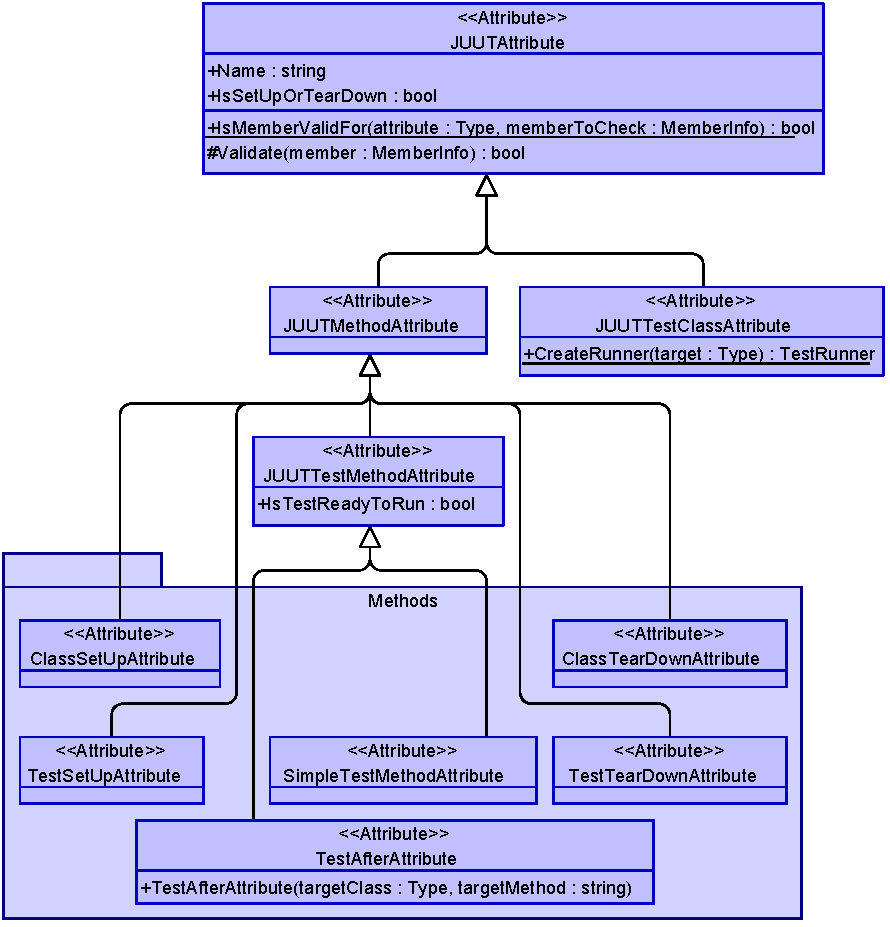
\includegraphics[width=0.9\linewidth]{images/Kapitel_Ergebnis/Attributes}
\caption[Attribute zur Markierung testspezifischer Elemente]{Attribute zur Markierung testspezifischer Elemente}
\label{fig:Attributes}
\end{figure}

Das \textit{JUUTTestClass}-Attribut wir zur Markierung von Testklassen benutzt. Zusätzlich zu den geerbten Funktionalitäten, liefert es auch den optimalen \textit{TestRunner} für die markierter Testklasse. Denn je nachdem welche Arten von Tests diese enthält wird ein anderer Typ \textit{Runner} zur fehlerfreien Ausführung benötigt.

Als abstrakte Superklasse aller Testmethoden dient \textit{JUUTTestMethodAttribute}. Dadurch kann einem der \textit{TestClassScanner} alle Tests einer Testklasse liefern, ohne alle konkreten Test-Attribute zu kennen. Es hat ein öffentlich lesbares Attribut \textit{IsReadyToRun} welches angibt, ob der markiert Test schon ausgeführt werden kann. Dies wird von den \textit{Runnern} berücksichtigt, wodurch komplexere Testmethoden möglich sind. Für konkrete Tests gibt es die Attribute \textit{SimpleTestMethod} und \textit{TestAfter}. Mit Ersterem markiert man einfache Tests, die immer bereit zur Ausführung sind. Diese sind äquivalent zu den Tests die mit UUnit oder SharpUnit möglich sind. Mit \textit{TestAfter} versehene Tests sollen nach der Ausführung einer bestimmten Methode einer Klasse durchgeführt werden (zum Beispiel die \textit{Update}-Methode eines Skripts). Ursprünglich hatte ich vor diese Funktionalität mit Aspektorientierte Programmierung\footnote{Mit AOP lassen sich eigene Funktionalitäten an bestimmte Stellen des Programms einweben. Mehr dazu findet man zum Beispiel in \textit{"`Aspect-oriented programming"} unter anderem von Gregor Kiczales.} zu implementieren. Das Attribut wäre dabei gleichzeitig der \textit{Advice} der nach dem Methodenaufruf eingewoben werden würde und einen \textit{ReadyToRun}-Flag auf wahr setzt, wodurch der \textit{Runner} den Test beim nächsten Durchgang ausführt. Allerdings wird zum Umweben einer nicht statischen Methode einer Klasse ein \textit{Proxy-Objekt} benötigt, welches an Stelle des eigentlichen Objekts verwendet wird. Leider ist es nicht möglich in einer laufenden Unity-Umgebung ein Skript durch ein entsprechendes \textit{Proxy-Objekt} zu ersetzen. Zum Zeitpunkt der Fertigstellung dieser Studienarbeit war es mir nicht möglich dieses Problem zu lösen, sodass diese Funktionalität nur schematisch vorhanden ist.

Neben Attributen für Testmethoden, gibt es noch weitere für \textit{SetUp}- und \textit{TearDown}- Methoden. Von der Definition von Tests entspricht JUUT also dem Funktionsumfang von MSTest.

Abgesehen von den Attributen sind für Tests noch die möglichen Assertions wichtig. Diese werden von der Klasse \textit{Assert} zur Verfügung gestellt.
\begin{wrapfigure}{r}{0.5\linewidth}
\centering
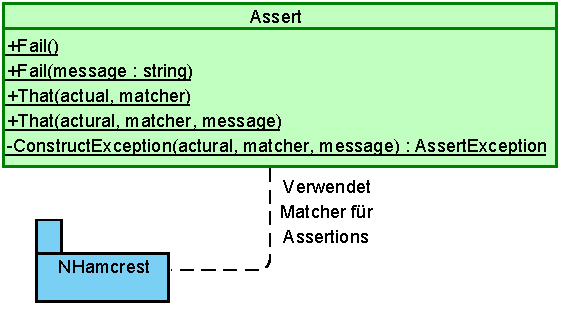
\includegraphics[width=0.95\linewidth]{images/Kapitel_Ergebnis/Assert}
\caption[\textit{Assert}-Klasse von JUUT]{\textit{Assert}-Klasse von JUUT}
\label{fig:Assert}
\end{wrapfigure}
Durch die Verwendung von NHamcrest ist diese sehr schlank und bietet dennoch mehr Bedingungen, auf die getestet werden können, als die Standard-\textit{Assert}-Klassen von UUnit, SharpUnit oder MSTest. So werden nur zwei Methoden benötigt. Zum einen die Methode \textit{Fail}, die den Test gezielt fehlschlagen lässt, indem sie eine \textit{AsserException} wirft. Optional lässt sich diese mit einer Nachricht versehen, welche bei der Präsentation angezeigt wird. Dazu kommt noch die Methode \textit{That}. Diese erwartet das zu überprüfende Objekt \textit{actual} und einen \textit{Matcher}, der überprüft ob dieses eine bestimmte Bedingung erfüllt. Bedingungen können sein, dass \textit{actual} nicht Null ist oder dass von einer Anweisung eine Exception geworfen wird.

Abschließend wird gezeigt, wie ein Test mit JUUT definiert werden kann:
\begin{lstlisting}[caption={[Beispiel für einen Test mit JUUT]Beispiel für einen Test mit JUUT\\In diesem Fall sind \textit{Throws.An} und \textit{Is.NotNull} die Matcher, welche den ersten Parameter darauf überprüfen, dass eine Exception geworfen wird beziehungsweise das Objekt nicht Null ist.}, label=code:SimpleTestMethodAttribute_Validate]
[JUUTTestClass]
public class TestClass {
	
	private ClassToTest objectToTest;
	
	[TestSetUp]
	public void SetUp() {
		objectToTest = new ClassToTest();
	}
	
	[SimpleTestMethod]
	public void TestObjectCreation() {
		Assert.That(() => { new ClassToTest(null); }, Throws.An<ArgumentException>());
		Assert.That(objectToTest.ImportantProperty, Is.NotNull());
	}
		
	[TestSetUp]
	public void SetUp() {
		objectToTest = null;
	}
	
}
\end{lstlisting}
\clearpage

\subsection{Ausführen der Tests}

Das Ausführen der Tests ist die Kernfunktionalität eines Test-Frameworks und wird bei JUUT von den Paketen \textit{Sessions}, \textit{Runners} und \textit{Suites}, unter der Zuhilfenahme der \textit{Scanner}, durchgeführt. Die \textit{Sessions} verwalten die auszuführenden Tests, während \textit{Runner} und die \textit{Suite} für das tatsächliche Testen zuständig sind.

Als erstes muss der Anwender mit \textit{Session}-Objekten definieren, welche Tests durchgeführt werden sollen, weswegen dieses Paket zuerst vorgestellt wird.

\begin{figure}[h]
\centering
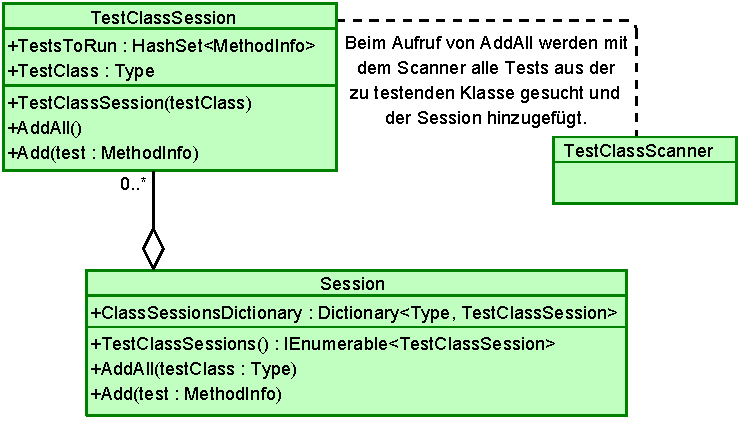
\includegraphics[width=0.8\linewidth]{images/Kapitel_Ergebnis/Sessions}
\caption[\textit{Sessions}-Paket]{\textit{Sessions}-Paket}
\label{fig:Sessions}
\end{figure}

Eine \textit{TestClassSession} repräsentiert eine Testklasse und verwaltet die zu dieser Klasse gehörenden Testmethoden. Sie muss einer mit dem \textit{JUUTTestClass}-Attribut versehenen Klasse zugeordnet werden, weswegen sie als Konstruktor-Parameter einen Typ erwartet. Mit den Methoden \textit{AddAll} und \textit{Add} können alle oder einzelne Testmethoden der Testklasse hinzugefügt werden. Beim Aufruf von \textit{AddAll} durchsucht die statische Hilfsklasse \textit{TestClassScanner} den zugeordneten Typ nach Methoden, welche mit einem \textit{JUUTTestMethod}-Attribut markiert wurden, die dann zur \textit{Session} hinzugefügt werden. Wie das Scannen genau implementiert wurde, sieht man in der Sektion \ref{sec:Appendix_Scanners} \nameref{sec:Appendix_Scanners} im Appendix.

\textit{TestClassSession} dient der JUUT-internen Verwaltung. Vom Anwender muss lediglich eine \textit{Session} erzeugt werden, welche wiederum eine Menge von \textit{TestClassSessions} verwaltet. Diese werden in Form einer Hashtabelle gespeichert, wobei der Schlüssel der Typ der Testklasse und das Element die dazugehörige \textit{TestClassSession} ist. Die Methoden \textit{AddAll} und \textit{Add} von \textit{Session} überprüfen nun, ob es schon eine \textit{TestClassSession} für den hinzuzufügenden Test gibt, erstellen gegebenenfalls eine Instanz und delegieren dann an das \textit{TestClassSession}-Objekt. Die Definition einer \textit{Session} könnte wie folgt aussehen:
\begin{lstlisting}[caption={[Beispiel für die Definition einer \textit{Session}]Beispiel für die Definition einer \textit{Session}}, label=code:Example_SessionCreation]
Session session = new Session();
session.AddAll(typeof(TestClass));
session.Add(typeof(AnotherTestClass).GetMethod("ATestMethod"));
\end{lstlisting}

Nachdem eine \textit{Session} definiert wurde, müssen die darin enthaltenen Tests ausgeführt werden. Diese Aufgabe übernimmt die \textit{TestSuite} und weitere Klassen, welche im nachfolgenden Klassendiagramm dargestellt sind.

\begin{figure}[h]
\centering
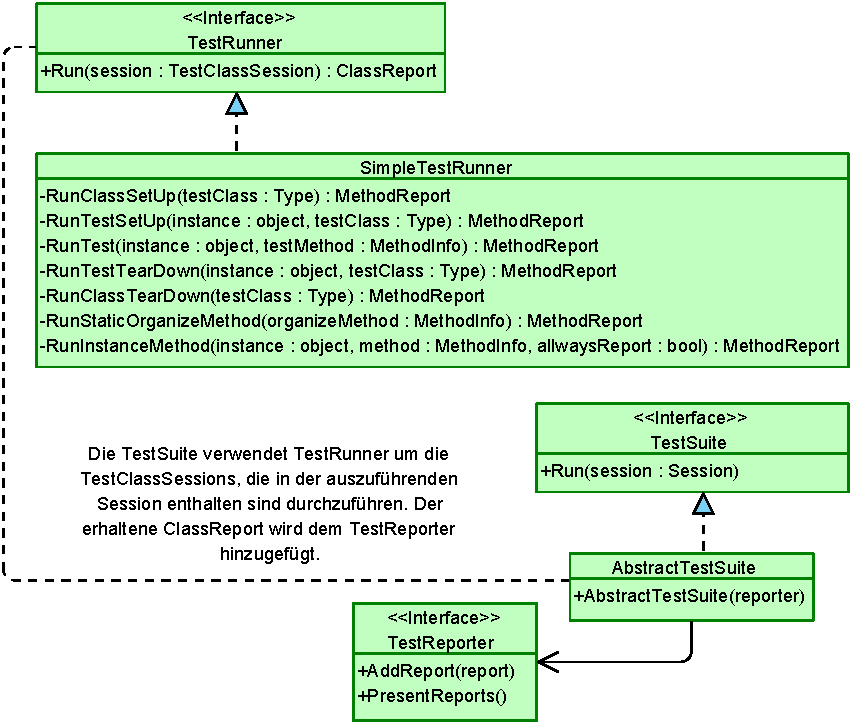
\includegraphics[width=0.8\linewidth]{images/Kapitel_Ergebnis/SuitesAndRunners}
\caption[Für die Ausführung von Tests verantwortliche Klassen]{Für die Ausführung von Tests verantwortliche Klassen}
\label{fig:SuitesAndRunners}
\end{figure}

Eigentlich führen die \textit{TestRunner} die Tests durch, da die \textit{TestSuite} für jede in der \textit{Session} enthaltene \textit{TestClassSession} an einen \textit{TestRunner} delegiert. Der zurückgegebene \textit{ClassReport} wird dem \textit{TestReporter} hinzugefügt und nach Abschluss wird dessen \textit{PresentReports}-Methode aufgerufen um die Ergebnisse darzustellen. Der Ablauf innerhalb des \textit{TestRunners} ist wie folgt:
\begin{enumerate}
\item Erzeugung einer \textit{ClassReport}-Instanz
\item Aufruf der \textit{ClassSetUp}-Methode
\item Erzeugung einer Instanz der zu testenden Klasse
\item Für jeden Test der \textit{TestClassSession}
	\begin{enumerate}[label*=\arabic*.]
	\item Aufruf der \textit{TestSetUp}-Methode
	\item Aufruf der Testmethode
	\item Aufruf der \textit{TestTearDown}-Methode
	\end{enumerate}
\item Aufruf der \textit{ClassTearDown}-Methode
\item Rückgabe des gefüllten \textit{ClassReports}
\end{enumerate}

Die einzelnen Methodenaufrufe werden mit Hilfe von \textit{Reflection} durchgeführt. Falls dabei eine Exception geworfen wird, wird diese gefangen und daraus ein \textit{MethodReport} erzeugt, welcher der \textit{ClassReport}-Instanz hinzugefügt wird. Tritt ein Fehler in einer der organisierenden Methoden (z.B. \textit{TestSetUp} oder \textit{TestTearDown}) auf, wird der Durchlauf abgebrochen und der Bericht sofort zurückgegeben, da der Fehler bei jeder einzelnen Testmethode auftreten würde. Die konkrete Implementierung findet man in der Sektion \ref{sec:Appendix_Runners} \nameref{sec:Appendix_Runners} im Appendix.

Eine \textit{Session} lässt sich nun mit folgendem Code ausführen:
\begin{lstlisting}[caption={[Beispiel für die Ausführung einer \textit{Session}]Beispiel für die Ausführung einer \textit{Session}\\\textit{ConcreteTestSuite} ist stellvertretend für eine beliebige Implementierung von \textit{AbstractTestSuite}.}, label=code:Example_SessionCreation]
Session session = new Session();
session.AddAll(typeof(TestClass));
session.Add(typeof(AnotherTestClass).GetMethod("ATestMethod"));

TestSuite suite = new ConcreteTestSuite();
suite.Run(session);
\end{lstlisting}
\clearpage

\subsection{Präsentation der Testergebnisse}

Nachdem die Tests durchgeführt wurden, müssen die Ergebnisse nur noch dem Benutzer präsentiert werden. Da die Form der Präsentation abhängig von der Spiele-Engine ist, worauf in \autoref{sec:Ergebnis_Unity} näher eingegangen wird, beschäftigt sich dieser Teil mit der Strukturierung und Verwaltung der einzelnen Berichte.

\section{Unity}
\label{sec:Ergebnis_Unity}

\section{Zusammenfassung}
	\chapter{Fazit}

Zeilen source code
Tests Robustheit, Erweiterbarkeit, Usability
	
	% Anhang
	\clearpage
	\pagenumbering{roman}

	% Abbildungsverzeichnis
	\cleardoublepage
	\phantomsection \label{listoffig}
	\addcontentsline{toc}{chapter}{Abbildungsverzeichnis}
	\listoffigures

	% Quellcodeverzeichnis
	\cleardoublepage
	\phantomsection \label{listoflist}
	\addcontentsline{toc}{chapter}{Listings}
	\lstlistoflistings

	% Literaturverzeichnis
	\cleardoublepage
	\phantomsection \label{listoflit}
	\addcontentsline{toc}{chapter}{Literaturverzeichnis}
	\begin{thebibliography}{---}

\bibitem[FRE10]{FRE10}
  \textsc{Steve Freeman und Nat Pryce}: 
  \textbf{Growing Object-Oriented Software, Guided by Tests}.
  2010, Addison-Wesley Professional, S. 1-67
    
\bibitem[HEN10]{HEN10}
  \textsc{Ryan Henson Creighton}
  \textbf{Unity 3D Game Development by Example: Beginner's Guide}.
  2010, Packt Publishing
      
\bibitem[TDGD13]{TDGD13}
  \textsc{Jonas Goldt und Lennart Hensler}
  \textbf{Test Driven Game Development mit Unity 3D}.
  2013, Studienarbeit DHBW Karlsruhe

\end{thebibliography}



	% Abkürzungsverzeichnis
	% vorher in Konsole folgendes aufrufen: 
	%	makeglossaries makeglossaries dokumentation.acn && makeglossaries dokumentation.glo
	\printglossary[type=\acronymtype]
	
	% Glossar
	\printglossary[style=altlist,title=Glossar]
\end{document}

